%% chapter of SNO+ detector

%%\epigraph{There is an art in the contemplation of water. It is necessary to look at it as foaming in waves.}{--- \textup{Mencius}, \textit{\\translated by James Legge}}

\section{Overview}\label{An Overview of SNO+}
The SNO+ experiment is located at SNOLAB in Vale's Creighton mine in Sudbury, Ontario, Canada (coordinate: 46$^\circ$28'19.6"N, 81$^\circ$11'12.4"W). The deep underground facility of the SNOLAB provides an environment with extremely low cosmic ray backgrounds. At sea level, an average cosmic muon ($\mu$) flux rate is about $1.44\times 10^7~\mu/m^2/day$l\cite{muonflux}. Cosmic muons with high energies ($\mathcal{O}(GeV)$) can induce spallation backgrounds, such as fast neutrons and lasting isotopes, which are harmful to the low background counting experiments\cite{beacom2017physics}. The SNOLAB has a $2092\pm6$ m flat overburden of rock, which is $5890\pm94$ water equivalent meter (m.w.e). This rock overburden ensures that cosmic muon ($\mu$) flux rate is as low as $0.286\pm0.009~\mu/m^2/day$, which means that every hour only about 1 $\mu$ passes through the SNO+ detector. 

The SNO+ detector is the successor of the SNO experiment. The detector makes use of the SNO structure and has been upgraded. The detector consists of an acrylic vessel (AV) sphere of 12 m in diameter and 5.5 cm in thickness. The AV sphere is concentric within a stainless steel photomultiplier(PMT) support structure (PSUP), which is a geodesic dome with an average radius of 8.4 m. The Hamamatsu 8-inch R1408 PMTs are mounted on the PSUP. 9394 PMTs are looking inward to the AV, giving a 50\% effective coverage, while 90 PMTs are looking outward, serving as muon vetos. These two structures are housed in a rock cavity filled with 7000 tonnes of ultrapure water (UPW) to provide both buoyancy for the vessel and radiation shielding of the surrounding backgrounds, such as the cosmic rays and isotope decays from the rock.

%
\begin{figure}[htbp]
	\centering
	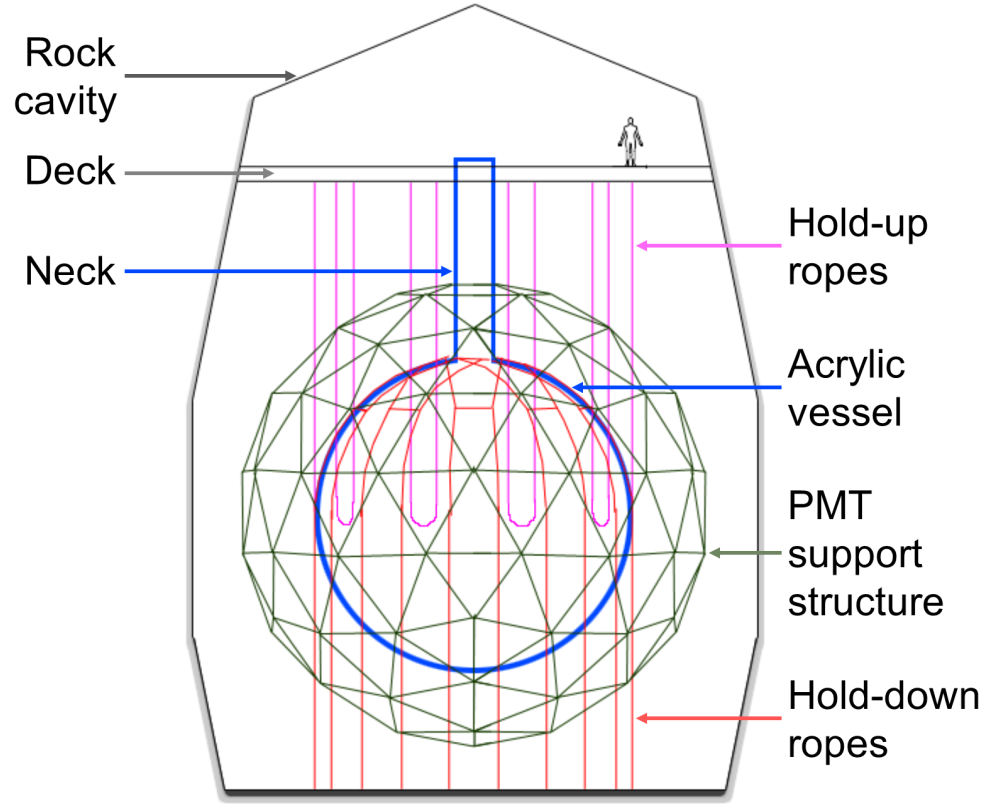
\includegraphics[width=10cm]{SNOPdetector.png}
	\caption{The SNO+ detector labelled with main structures, figure modified from \cite{mekarski2018electron}; the original version is from \cite{jones2011background}}.
	\label{snopdetector}
\end{figure}


main upgrades from SNO to SNO+
BiPo tagging on partial fill data


The detector has been running since December 2016.
\cite{anderson2019search},

\section{SNO+ Physics Phases}
The SNO+ detector is designed for multi-purpose measurements of neutrino physics.
The experiment will go through three phases\cite{whitepaper}: 

1. Water phase 

The AV was filled with about 905 tonnes of ultra pure water (UPW). The detector has been collecting physics data since May 2017.

The main physics goal in this phase is to search for the invisible nucleon decay, which violates baryon number and is a prediction of Grand Unified Theory (GUT). In this decay mode, $^{16}$O decays into $^{15}$O$^*$ or $ ^{15}$O$^*$, which de-excites and produces a $\gamma$ ray of about 6 MeV.

During the water phase, different types of calibration runs have been taken. The detector responses, systematics and backgrounds are studied. Multiple physics analyses of solar neutrinos, reactor antineutrinos and nucleon decay are going on. The external backgrounds are also measured, which will be the same as the following two phases. 

2. Scintillator phase

The AV will be filled with 780 tonnes of liquid scintillator, which is a mixture of linear alkylbenzene (LAB) as a solvent and 2 g/L of 2,5-diphenyloxazole (PPO) as a fluor.

In this phase, the main physics goal is to measure low energy solar neutrinos: the CNO, pep and low energy $^8$B neutrinos. The pep neutrinos are mono-energetic, with $E_\nu$=1.442 MeV and their flux is well predicted by the Standard Solar Model. A measurement of the pep neutrinos will give more information of the matter effects in neutrino oscillations\cite{borexino}. 

The solar metallicity is the abundance of elements heavier than $^4$He (called ``metal'' elements in the context of astronomy). It is poorly constrained and the predictions from different solar models disagree with each other. A measurement of the CNO neutrinos can give the abundance of $^{12}$C, $^{13}$N and $^{15}$O and can thus resolve the metallicity problem\cite{cno}.

Geoneutrino, reactor antineutrino and supernova neutrino detections are additional goals.

A six-month period of scintillator filling and six to twelve months of data-taking are expected for this phase. During the filling, it is planned to operate the partially filled detector at a water level about 4.4 m for about two weeks. This partial filled transition phase is mainly aimed to understand the in-situ backgrounds of scintillator. 

3. Tellurium loading phase

In this final phase, 0.5\% natural Tellurium by mass will be loaded into the scintillator.
Higher loading concentrations would be possible for a further loading plan\cite{Paton:2019kgy}.
 The $^{130}$Te is a double beta decay isotope. The main purpose in this phase is searching for $0\nu\beta\beta$ in $^{130}$Te.


\section{Detection Medium}
In the SNO+ detector, charged particles are expected to interact with the detection medium and create Cherenkov lights and scintillation lights. 

\subsection{Cherenkov Radiation}
For any charged particle travelling in a transparent medium at an ultrarelativistic speed (a speed greater than the local phase speed of light in the medium), an electromagnetic radiation, called Cherenkov radiation, can be emitted from the coherent response of the medium under the action of the field of the moving particle\cite{jackson2007classical,landau2013electrodynamics}.

Suppose a charged particle moves in a transparent, isotropic and non-magnetic medium and creates an electromagnetic wave. The electromagnetic wave propagates with a wave number $k=n\cdot\omega/c$, where $c$ is the speed of light in vacuum, $n$ is the real-valued refractive index and $\omega$ is the frequency. If the particle travels uniformly along x axis with a velocity of $v$, the x-component of the wave vector is $k_x=\omega/v$. For a freely propagating wave, $k>k_x$, therefore $v>v_p=c/n(\omega)$, where $v_p$ is the phase velocity in the medium. Under this condition that the speed of the charged particle is greater than the $v_p$, the Cherenkov radiation is emitted with a frequency of $\omega$\cite{landau2013electrodynamics}.   

The Cherenkov angle, $\theta_c$ is the angle between the direction of the particle and the direction of Cherenkov emission and it is well-defined by $\cos\theta_c(\omega) = \frac{c}{n(\omega)v}$. The radiation is distributed over a surface of a cone with the half-opening angle $\theta_c$. 

Consider the condition $v>v_p=c/n(\omega)$, for the case of $e^-$ travelling in a water detector, if neglecting the dependency on $\omega$, $n_{water}\simeq 1.33$ \cite{pdg2018}, then $\theta_c\simeq 41.25^\circ$ and $v_p\simeq 2.254\times10^8~m/s$, which corresponds to a kinetic energy $E_k=(\gamma-1)mc^2=0.264~MeV$ for $e^-$, where $\gamma=1/\sqrt{1-v_p^2/c^2}$. This is the lowest kinetic energy to create Cherenkov radiation, which is referred to the Cherenkov threshold ($E_{thresh}$). In the case that the LAB-PPO liquid scintillator is the medium, $n\simeq 1.50$\cite{tseung2011ellipsometric}, $\theta_c\simeq 48.19^\circ$ and for $e^-$, $E_{thresh}\simeq 0.175~MeV$.   

For a particle with a charge of $ze$, the number of photons produced by Cherenkov radiation per unit path length and per unit frequency of the photons is given by\cite{leo2012techniques}:
\[
\frac{d^2N}{d\omega dx}=\frac{\alpha^2 (ze)^2}{c}\sin^2\theta_c=\frac{z^2\alpha}{c}(1-\frac{1}{\beta^2 n^2(\omega)}),
\]
where $\alpha$ is the fine structure constant.

Translate the frequency into the wavelength ($\lambda=2\pi\omega$) and integrate over the wavelength, we have the number of photons and $x$ is along the particle track\cite{leo2012techniques}:
\[
\frac{dN}{dx}=2\pi (ze)^2\alpha\sin\theta_c\int_{\lambda_1}^{\lambda_2}\frac{d\lambda}{\lambda^2},
\]

For optical photons with wavelengths ranging from $350$ to $550~nm$ (typical PMT detection sensitive range), the above formula can be calculate into\cite{leo2012techniques}:
\[
\frac{dN}{dx}=476(ze)^2\sin^2\theta_c~photons/cm.
\]

For the Cherenkov radiation caused by $e^-$ in a water detector, $dN/dx \simeq 207~photons/cm$; while in the LAB-PPO case: $dN/dx \simeq 264~photons/cm$. In a realistic measurement, the detection efficiency and the coverage of photon sensors are also required to be taken into account.

\subsection{Scintillation from Organic Scintillator}

Besides the Cherenkov photons described in the last section, the majority lights emitted from organic scintillator are scintillation photons.

The organic liquid scintillator can convert the kinetic energy of charged particles into scintillation photons with wavelengths in the sensitive detection region of PMTs. They are aromatic hydrocarbon compounds with benzene-ring structures. When ionizing radiation happens in the scintillator, the free valence electrons of the molecules are excited and transit to occupy the $\pi$-molecular orbitals with the benzene rings. These highly delocalized electrons are called $\pi$-electrons, which can occupy a series of energy levels. A Jablonski diagram, invented by Polish physicist Aleksander Jab\l o\'{n}ski, is generally used to describe molecular absorbance and emission of light. In Fig.~\ref{jablonski}, the Jablonski diagram illustrates the $\pi$-electronic energy levels of an organic scintillator molecule\cite{knoll2010radiation,leo2012techniques}. 
\begin{figure}[!htb]
	\centering
	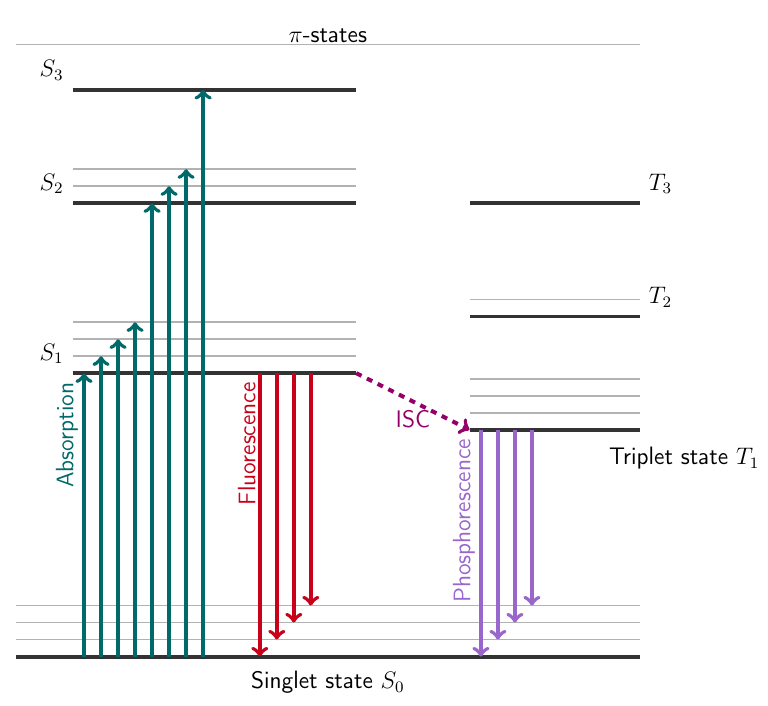
\includegraphics[width=10cm]{jablonski.png}
	\caption{A Jablonski diagram for the organic scintillator, modified from \cite{birks1965theory, knoll2010radiation}.}
	\label{jablonski}
\end{figure}

In the diagram, $S_{0,1,2,3,...}$ are the energy levels of the spin-0 singlet states, where $S_0$ is the ground state and $S^*=S_{1,2,3,...}$ are the excited singlet states. Above the ground state $S_0$, there are also a set of spin-1 triplet states $T_{1,2,3,...}$, where $T_1$ is the lowest triplet state. These electron energy levels are labelled with thick black lines. The energy spacing between these levels are $\mathcal{O}(eV)$. In each levels, there are also fine structure levels which corresponds to excited vibration modes of the molecule (labelled with gray lines and can be marked as $S_{10}, S_{11}, ..., S_{20},S_{21}, ...$). The energy spacing between these fine levels are $\mathcal{O}(0.15~eV)$\cite{leo2012techniques, knoll2010radiation}.

The ionization radiation transfers the energy to the molecules and excites the electron levels as well as the vibrational levels, labelled as the absorption lines (in green). The decays between the excited singlet states (not to the ground state) are almost immediate ($\leq 10~ps$) without the emission of light. This process is called internal degradation. The decays from the excited singlet state $S_1$ (as well as the vibrational states $S_{10},S_{11},S_{12},...$) to the ground state (as well as the vibration states $S_{01}, S_{02}, ...$) happen promptly ($\mathcal{O}(ns)$) and emit lights (labelled as red lines). This process is called fluorescence which contributes the prompt component of the emission of scintillation light. The probability of $S_1$ decays into the vibrational states $S_1 \to S_{01},S_{02},...$ among the ground state is more than $S_1\to S_0$. Since the absorbed energy of $S_0 \to S_1$ is larger than the emitted energy of $S_1 \to S_{01},S_{02},...$, the scintillators have very little self-absorption of the fluorescence and are transparent to their own radiation. The effect of Stokes shift, which refers to the overlap between the optical absorption and emission spectra, is small for the organic scintillator\cite{leo2012techniques,knoll2010radiation}. 

The transitions between the singlet and triplet states are highly forbidden due to the
electron spin-flip is involved\cite{von2015measurement,sorensen2016temperature}. There also exists a relatively rare process called intersystem crossing (ISC), which converts excited singlet states into triplet states. Besides this, 75\% of triplet states can be produced by ionization-recombination\cite{von2015measurement,dunger2018topological}.

For the de-excitation, the similar processes of internal degradation occur among $T_{2,3, ...} \to T_1$. $T_1$ is a relatively stable state and the lifetime of the molecule in the triplet state is in $\mathcal{O}(10^{-4}~-~10~s)$\cite{mcquarrie1997physical}. $T_1\to S_0$ is highly forbidden. However, the $T_1$ state can go through an indirect decay process by interacting with another excited $T_1$ molecule and forms an excited singlet state:
\[
T_1+T_1\to S^*+S_0+phonons
\]
The $S^*$ will de-excite and emit delayed scintillation light. The process for emitting this delayed scintillation light is called delayed fluorescence or phosphorescence\cite{leo2012techniques}. This process contributes to the delayed component of scintillation light.

For a typical scintillator detector, the time scale of detector response is $\mathcal{O}(1-100~ns)$. In this time region, the emission of the scintillation light contains the primary fluorescence from the de-excitation of the singlet states (prompt component) and the delayed fluorescence from the de-excitation of the indirect triplet states (delayed component)\cite{dunger2018topological}. The time profile of the scintillation light emission is a mixture of prompt and delayed components. 

Different charged particles can cause different ionization density when they deposit energies to the scintillator molecules. The ionization density affects the relative population of the excited singlet and triplet states. Compared to an $e^-$, an $\alpha$ particle can cause a high ionization density, which produces higher ratio of triplet states. Therefore, the time profile for the $\alpha$ particle has more delayed component or longer tails than the $e^-$. This enables the organic scintillator to distinguish $\alpha$ with $e^-$ or other lighter charged particles\cite{dunger2018topological, scintillatorPaper}. 





an empirical formula, called follows Birk's law\cite{birks1951scintillations, birks1965theory}, describes the photon yield along unit distance by the incident particle:
\[
\frac{dY}{dx}=A\frac{dE/dx}{1+k_B\cdot dE/dx},
\]
where $A$ is a normalization constant, $k_B$ is the Birks' constant of the scintillator, which in practice is obtained by fitting the formula to the measured data.




\subsection{Liquid Scintillator for SNO+}

The SNO+ collaboration has been developing liquid scintillator 

Linear Alkyl Benzene (LAB)

is provided by CEPSA Qu\'{i}mica B\'ecancour Inc.
Organic liquid scintillators 
The advantages of LAB are:

\begin{itemize}
	\item[$\bullet$] It has very low levels of natural radioactive contaminants such as U, Th and K.
	\item[$\bullet$] High light yield and attenuation length.
	\item[$\bullet$] It has fast timing response 
	different timing spectrum for $\alpha$ and $\beta$ events, which enables an $\alpha-\beta$ discrimination. 
	\item[$\bullet$] High flash point and low toxicity for lab safety.
	\item[$\bullet$] appropriate density for mechanical stability
	\item[$\bullet$] Good stability and chemically compatible with detector materials, mainly the AV.
	\item[$\bullet$] Low cost.
\end{itemize}


An additional wavelength shifter, 2,5-diphenyloxazole (PPO) is usually added and dissolved into the LAB \cite{wunderly1990new}. This wavelength shifter is used as a fluor and it can shift the wavelengths of the scintillation photons to a range of 300-550 nm, which is the sensitive range of the PMT detection.  A 2 g/L PPO concentration in LAB is optimized by SNO+\cite{whitepaper}. The absolute light yield of the LAB-PPO liquid scintillator has been well-measured from large particle physics experiments [cite dayabay, borexino] as well as bench-top measurements [cite dayabayBench, novikov, tanner]. The absolute light yield of LAB+2g/L PPO liquid scintillator determined by SNO+ is 11900 photons/MeV [cite lightyield].



Te-loaded liquid scintillator (TeLS)

To load the tellurium into the liquid scintillator, a compound is made by 
condensation reactions between telluric acid (TeA) and 1,2-butanediol (BD), with N,N-dimethyldodecylamine (DDA) being used as a stabilization agent.

A tertiary amine (N,N-Dimethyldodecylamine, DDA) was added during the reaction to stabilize TeBD complexes and avoid any phase separation. 




Tellurium-loaded 65\% of the pure, unloaded scintillator



water-based wavelength shifter


timing profile, the intensity of scintillation light as a function of time

the prompt fluorescence intensity at a time $t$ excitation be $I=I_0e^{-\frac{t}{\tau}}$



singlet and triplet states 
ionization density 
depend
$\alpha$-particle
high ionization density 
quenching, 




2 g/L PPO gives an absolute light yield of 11900 photons/MeV.


for the partial-fill phase, 0.5 g/L PPO gives Measurements in 0.5 g/L showed a light yield of 52\% of 2 g/L,  
6190 photons/MeV\cite{tanner0p5,joshW1}.





\section{Optics}

Optical parameters

Winston cone



timing


attenuation

scattering


laser pulse diffuser, it can run with different wavelengths: 337, 365, 385, 420, 450 and 500 nm.
The laserball 

The acrylic of the AV is UV-transparent

\section{Trigger and Readout of the SNO+ Detector}

As mentioned in \ref{overview}, the Hamamatsu 8-inch R1408 PMTs, as photon sensors, are the basic detection elements for the SNO+ detector. 

The photons created from particle interactions in the detector propagate to the PMT sphere and may hit a certain PMT and strike on its photo-cathode, which is a thin caesium bialkali film coated on the inner surface of PMT glass. The photocathode then produces a photo-electron through photoelectric effect. The photocathode is set at ground voltage while the anode is at a high voltage ranging from $+1700$ to $+2100~V$ \cite{boger2000sudbury,dunger2018topological}. This forms electric fields inside the PMT. The photo-electron is accelerated and focused by the electric field in the PMT and goes through the volume which is under vacuum until it reaches the region of a series of secondary emission electrodes, called dynodes. The nine dynode strings are constructed in a Venetian blind configuration in R1408 PMT \cite{boger2000sudbury,leo2012techniques}. When the photo-electron transfers its energy to the materials in dynodes, a number of secondary electrons escape and form a measurable current which is collected by the a custom-made operating circuit (PMT base) at the anode \cite{hamamatsu2018photomultiplier}.

19 crates$\times$16 Front End Cards (FEC)$\times$32 channels = 9728 electronics channels.


The PMT hit time of 


Once the global trigger signal is issued, the integrated charges and time from an event are stored in each channel.

\cite{rattime,bonventre2014neutron}





Each crate processes 16$\times$32 = 512 PMTs.
9605 channels are actually used and among them, 32 channels are reserved for calibration devices and labelled as FEC Diagnose (FECD) channels


During the experiment running, the maintenance of the electronics is always ongoing.

crate controller card (XL3)


analog master trigger system (MTC/A+) 
("+" means an upgrade to SNO MTC/A)


digital master trigger system (MTC/D)

the analog waveforms are summed on the MTC/A+ card, then they are digitized 

CAEN v1720 digitizer 

TUBii trigger utility board 
pulsers and delays

DAQ 


nearline provides a real-time analysis of the data quality, 

trigger system
PMT Interface Card (PMTIC)
Front End Card (FEC)

NHit20 (N20), NHit100 (N100) trigger pulses.

MTC/A has 3 discriminators: LOW, MED and HI.

Global Trigger (GT)
the timing and charge from the fired PMT is digitized and stored.




Nhit means the number of live hit PMTs in the detector for a given event.


dark noise rate is estimated to be 1 kHz.


For the SNO+ detector specifically, each PMT that triggers sends multiple
trigger pulses down the electronics chain, which then performs higher logic.
These include both a 93 ns long square pulse (N100) and a 48 ns square pulse
(N20) 

These widths are chosen to match the characteristic travel times
of photons across the detector. More specifically, the N100 width is chosen
such that a set of photons from a Cherenkov cone will result in overlayed PMT
pulses. The shorter N20 width limits this overlaying of PMT pulses to events
originating from the centre of the detector.
If the total height of either of these summed pulses passes a set thresh-
27
old value, a global trigger (GT) is issued. This global trigger defines an
event" within the detector and results in all the associated information being
saved. Multiple different trigger thresholds can be set. For example: N100Lo,
N100Med, N100Hi are triggers based on the N100 pulses, where each has a
different threshold value set. So it is possible, and likely, that an event within
the detector passes several of these trigger thresholds.
Additionally, the detector can trigger from the charge in the PMTs directly.
The voltage pulses from all of the PMTs are summed together (ESUM). If this
combined voltage trace drops below a threshold value (for example, ESUMHi,
ESUMLo), this can also issue a GT to the detector.
Figure 3.4 shows the event display of a typical muon event in the detector. Each individual PMT that triggered for that event is highlighted at its
position on the support structure. A muon event is characterized by the large
number of triggered PMTs. As with nearly all muons that pass through the
detector, it is traveling in a downward direction. This is seen in Figure 3.4 as
the excess of PMT charge (i.e. photons) in the bottom of the detector. As all
atmospheric muons traveling upwards would be attenuated by the Earth, the
small flux of upward-going muons are the result of neutrino interactions in the
rock surrounding the detector [56].
Figure 3.5 shows a more typical event. The circular pattern seen is produced
by the projection of the Cherenkov light cone onto the PMTs. With 24 triggered
PMTs, this event is considered a high-energy event within the detector. The
size of the pattern indicates that this event took place closer to the PMTs
traveling in an outward direction, specifically in the water between the acrylic
sphere and the PMTs.




 will cause an electrical signal in the form of
a voltage drop. If this is larger than a threshold value, the electronics of that
PMT sends a trigger pulse.




The SNO+ electronics system includes trigger and readout systems, which record the time and charge information of PMT signals. The system can measure signals with a nanosecond-level timing resolution and single-photon level charge resolution and handle a rate of several kHz for normal operations.


Charged particles within the SNO+ detector are detected through the light that
they produce. For the water phase of the experiment, the detector measures
Cherenkov light using PMTs. A photon incident on a PMT may strike its
photocathode and produce a photoelectron. This photoelectron, after passing
through the PMT’s dynode chain,


burst 
from supernova


PMTs are Hamamatsu model R1408.


a single RG59/U type 75 $\Omega$ coaxial cable


cables bundle into groups

connected to the Paddle Cards, 
PMT Interface Card (PMTIC) 
\cite{andyElectronics}

\section{Calibration}


Two kinds of calibration sources are used by SNO+: optical sources and radioactive sources. 
The optical sources are used to calibrate the PMT response and to measure the optical properties of the 


The radioactive sources are used to calibrate the energy 

reconstruction performances and uncertainties.
particle identifications



Calibration sources with known physics parameters: help to understand the detector response to the events and to make accurate measurements
Two types of SNO+ calibration sources: optical sources and radioactive sources Optical sources: phototube response, optical properties of the detector media Radioactive source: energy scale, resolution, systematic
uncertainties
$^{16}$N calibration source is one of the radioactive sources


Optical calibration  {\emph {in-situ}} 
\begin{itemize}  
	\item[$\bullet$] Timing module for the Embedded LED Light Injection Entity (TELLIE)
	
	light-emitting diode (LED)
	
	
	time calibration, time response 
	
	a precision of $\mathcal{O} (1~ns)$
	
	Blinky fibre optics nailed to the PSUP to calibrate stuff.
	
	
	
	\item[$\bullet$]  
	
	
	\item[$\bullet$] 
\end{itemize}


Calibration source

The $^{16}$N source
$^{3}$H$(p,\gamma)^{4}$He reaction.

the SNO+ Source Manipulator System (SMS)
is inherited from the SNO.

A Umbilical Retrieval Mechanism (URM) is used to send the source down to the inner vessel.

The sources are connected to the umbilical.

An umbilical encloses electrical cables, optical fibres and gas lines connected to the source.

A Universal Interface (UI) connecting the URM and the detector, 
Therefore, sealed environment, which 
ensures radon gas not leaking into the detector when deploying the source.

\section{Monte Carlo Simulation and the RAT Software}
The SNO+ collaboration has developed a software framework, called the Reactor Analysis
Tool (RAT), which integrates a Monte Carlo simulation of the SNO+ detector and event-based analysis tools (for online and offline event analysis) since the beginning of the program. This software was originally developed by Stan Seibert for Braidwood Collaboration for a generic KamLAND like detector. It is also used by the other astroparticle physics experiemnts, such as DEAP/CLEAN, CLEAR and potentially for Darkside-50\cite{rat}.

Geant4 Toolkit and
incorporates ROOT libraries for data handling and analysis.

The RAT Monte Carlo was originally developed for the Braidwood Collaboration
utilising software developed for a generic KamLAND like detector, called Generic Liquid Scintillator GEANT4 simulation (GLG4). It was branched and
developed into the specialist SNO+ version, starting in 2006/2007.

GLG4sim


Braidwood

combines both Monte Carlo simulation of the Braidwood detector with event-based analysis tasks, like reconstruction. The primary goals are:

Make it easy to analyze Monte Carlo-generated events as well as data from disk using the same software with only a few command changes. Even in the proposal R\&D phase, where there is no real data, this is still useful for dumping Monte Carlo events to disk to be analyzed by another job. When there is real data, being able to do the analysis with the same code path as was used on Monte Carlo is very reassuring.
Allow for a modular, user-controlled analysis of events. This includes allowing the user to selected which analysis tasks to perform (different fitters, pruning unneeded data from the event data structure, etc.). It should also be relatively straightforward for users to introduce their own code into the analysis process.
Separate analysis into small tasks which can be developed asynchronously by different people, yet integrated with minimal (or perhaps zero) pain.
Integrate into existing GEANT4 and GLG4sim efforts with a minimum of code duplication. As much as possible, RAT should be designed incorporate upgrades of these packages just by relinking. No cut and paste of code (mainly a question with GLG4sim).
Design

the detailed processes of data acquisition and trigger systems are \cite{whitepaper}.

\cite{ratManual}





